\subsection{UC6 - Creazione scaffalatura}
\begin{figure}[H]
  \centering
  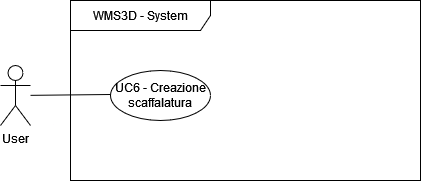
\includegraphics[width=0.8\textwidth]{UC_diagrams_1-10/UC6_sys.drawio.png}
   \caption{Diagramma UML UC6 - Creazione scaffalatura}
\end{figure}
\begin{figure}[H]
  \centering
  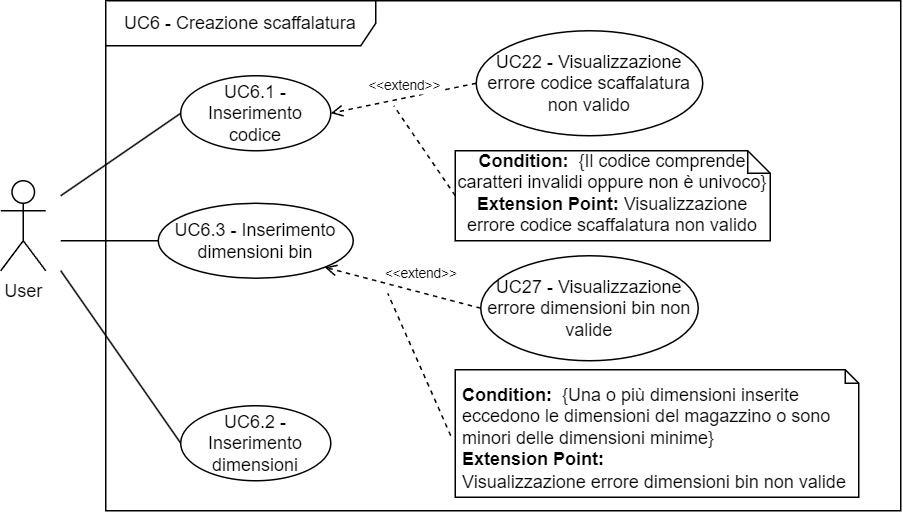
\includegraphics[width=0.8\textwidth]{UC_diagrams_1-10/UC6.drawio.png}
   \caption{Diagramma UML in dettaglio UC6 - Creazione scaffalatura}
\end{figure}
\begin{itemize}
    \item \textbf{Attori:} User.
    \item \textbf{Pre-condizione:}  L'utente ha creato/caricato un magazzino [UC1].
    \item \textbf{Post-condizione:} L'utente crea una scaffalatura, aggiunta in libreria, e che dovrà essere obbligatoriamente posizionata [UC7].
    \item \textbf{Scenario Principale:}  L'utente crea una scaffalatura, inserendo un codice univoco [UC6.1] e delle dimensioni [UC6.2].
    \item \textbf{Generalizzazioni:} -
    \item \textbf{Estensioni:} -
\end{itemize}


\subsubsection{UC6.1 - Inserimento codice}
\begin{itemize}
    \item \textbf{Attori:} User.
    \item \textbf{Pre-condizione:}  L'utente ha creato/caricato un magazzino [UC1] e vuole creare una nuova scaffalatura.
    \item \textbf{Post-condizione:} L'utente ha dato un codice identificativo per la nuova scaffalatura.
    \item \textbf{Scenario Principale:}  L'utente sceglie un codice univoco da dare alla scaffalatura.
    \item \textbf{Generalizzazioni:} 
    \item \textbf{Estensioni:} È presente una estensione nel caso in cui il codice non sia valido:
    \begin{itemize}
        \item UC22 - Visualizzazione errore codice scaffalatura non valido.
    \end{itemize}
\end{itemize}


\subsubsection{UC6.2 - Inserimento dimensioni}
\begin{figure}[H]
  \centering
  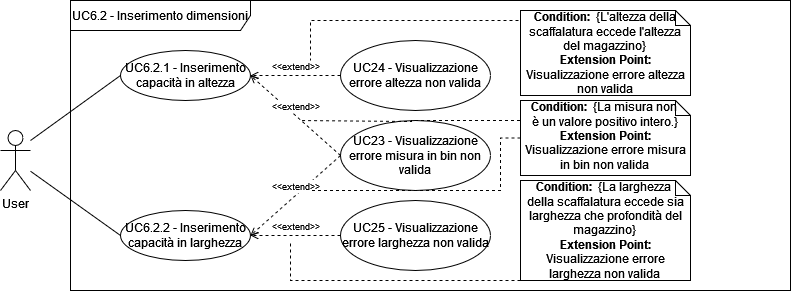
\includegraphics[width=0.8\textwidth]{UC_diagrams_1-10/UC6.2.drawio.png}
   \caption{Diagramma UML UC6.2 - Inserimento dimensioni}
\end{figure}
\begin{itemize}
    \item \textbf{Attori:} User.
    \item \textbf{Pre-condizione:} L'utente ha creato/caricato un magazzino [UC1] e vuole creare una nuova scaffalatura.
    \item \textbf{Post-condizione:}  L'utente ha inserito le dimensioni della nuova scaffalatura.
    \item \textbf{Scenario Principale:}  L'utente decide la capacità (numero di bin) in altezza e in larghezza da dare alla scaffalatura. Se le misure sono valide, la scaffalatura sarà creata.
    \item \textbf{Generalizzazioni:} -
    \item \textbf{Estensioni:} -
\end{itemize}


\paragraph{UC6.2.1 - Inserimento capacità in altezza}
\begin{itemize}
    \item \textbf{Attori:} User.
    \item \textbf{Pre-condizione:} L'utente ha creato/caricato un magazzino [UC1] e vuole creare una nuova scaffalatura.
    \item \textbf{Post-condizione:}  L'utente ha inserito la capacità in altezza della nuova scaffalatura.
    \item \textbf{Scenario Principale:}  L'utente decide il numero di bin in altezza da dare alla scaffalatura. 
    \item \textbf{Generalizzazioni:} -
    \item \textbf{Estensioni:} Sono presenti due estensioni:
    \begin{itemize}
        \item UC23 - Visualizzazione errore misura in bin non valida, nel caso in cui l'altezza non sia in un formato accettabile;
        \item UC24 - Visualizzazione errore altezza non valida, nel caso in cui l'altezza per la scaffalatura superi quella del magazzino.
    \end{itemize}
\end{itemize}


\paragraph{UC6.2.2 - Inserimento capacità in larghezza}
\begin{itemize}
    \item \textbf{Attori:} User.
    \item \textbf{Pre-condizione:} L'utente ha creato/caricato un magazzino [UC1] e vuole creare una nuova scaffalatura.
    \item \textbf{Post-condizione:}  L'utente ha inserito la capacità in larghezza della nuova scaffalatura.
    \item \textbf{Scenario Principale:}  L'utente decide il numero di bin in larghezza da dare alla scaffalatura.
    \item \textbf{Generalizzazioni:} -
    \item \textbf{Estensioni:}Sono presenti due estensioni:
    \begin{itemize}
        \item UC23 - Visualizzazione errore misura in bin non valida, nel caso in cui l'altezza non sia in un formato accettabile;
        \item UC25 - Visualizzazione errore larghezza non valida, nel caso in cui la larghezza per la scaffalatura superi quella del magazzino.
    \end{itemize}
\end{itemize}